\documentclass{scrartcl}

\usepackage{natbib}
\usepackage{hyperref}
\usepackage{amsmath}
\usepackage{verbatim}
\usepackage{listings}
\usepackage{color}
\usepackage{graphicx}


\usepackage{fvrb-ex}
\fvset{gobble=0,numbersep=3pt}
\fvset{numbers=left,frame=single}
%\RecustomVerbatimEnvironment{Verbatim}{Verbatim}{commandchars=§µ¶}
\DefineVerbatimEnvironment%
{CVerbatim}{Verbatim}
{fontfamily=tt,fontsize=\small,frame=single,formatcom=\color{blue},label=\emph{Interactive Stata example}}
\DefineVerbatimEnvironment{Sinput}{Verbatim}{fontshape=sl,formatcom=\color{blue}}


\lstset{ %
  basicstyle=\tiny\ttfamily\color{blue}, %
  frame=single, %
  includerangemarker = false, %
  title = \footnotesize\ttfamily\color{blue}\emph{Interactive Stata Example}, %
  captionpos = t, %
  rangeprefix=***, %
  %belowcaptionskip = -0.08in, %
  label={bla}
}

\lstnewenvironment{stata}
  {label=blabla}{}

\begin{document}

	\title{Homework assignment \#6\\ Panel Data Analysis}
	\subtitle{MPP-C6: Statistics 2}
	\author{Prof. Jan C. Minx\\ \texttt{minx@hertie-school.org} \\
		\url{http://moodle.hertie-school.org/course/view.php?id=1192}}
	\date{29 October 2015}
	
	\maketitle
	
	\indent\textbf{Disclaimer: This document sketches some brief responses to the questions of the homework assignment. It serves to provide students with some guidance. The document may include som flaws - those should be reported to me as students go through the responses.}

	\subsection*{Project Description}
	The Environmental Kuznets Curve is at the heart of a long-standing discourse on the relationship between economic development and environmental quality. It hypothesizes an inverted U-shape relationship between indicators of environmental degradation and per capita income. While some have used the EKC to argue that growth policies are also superior for dealing with environmental problems, others have questioned the existence of EKCs for different indicators or stressed very high turning points. We aim to reproduce the results of Stern and Common (2001) which sought to investigate the presence of an environmental Kuznets curve (EKC) for sulfur emissions \cite{stern2001there}.
	
	\subsection*{Dataset}
	The dataset stern2.dat contains country data from 1960-1990. The dataset contains the following variables
	\begin{itemize}
	\item \textit{year}: the year in which the country was observed 
	\item \textit{country}: numerical code that uniquely identifies each country (see table 1)
	\item \textit{gdpppp}: GDP per capita (purchasing power parity) in real 1990 international dollars
	\item \textit{pop}: population in 1000 residents
	\item \textit{so}: \(SO_2\) emissions in tonnes
	\item \textit{sopc}: \(SO_2\) emissions in tonnes per capita
	\item \textit{oe}: dummy variable describing oecd membership where 1000 represents membership and 2000 represents non-membership
	\end{itemize}
	
	\subsection*{Questions}
	
	\begin{enumerate}
	\item \textbf{Read the paper by Stern and Common. Explain the EKC hypothesis in your own words. What is the difference between sulfur and carbon emissions in the empirical discussion and why? What is the authors' perceived contribution to the discussion? What is the role of panel data therein? [conceptual question]}
		
	\item \textbf{Start by examining your data. Try out some descriptive statistics of the xt command family and report relevant ones. What sort of distribution do our variables of interest display? What transformations could we apply to the data? If necessary, create new variables that are appropriately transformed.}
	
	\lstinputlisting[linerange={lstart-lend}]{../stata/stern_assignment_q2.log}
	
	\item \textbf{Plot GDP per capita against sulfur emissions per capita (transformed if necessary). Describe the relationship you can see.}
	
	\lstinputlisting[linerange={lstart-lend}]{../stata/stern_assignment_q3.log}
	
	 \begin{figure}
      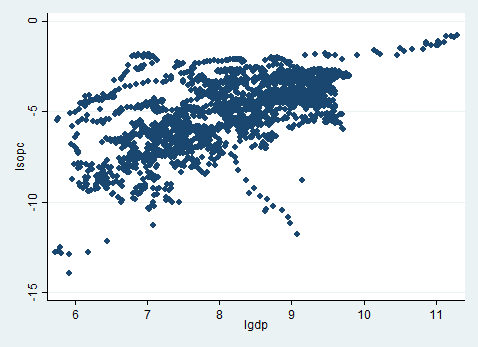
\includegraphics[width=12cm]{../stata/lsopc_lgdp.png}
      \caption{log GDP per capita against log sulfur emissions per capita}
    \end{figure}
	
	\item \textbf{Write the equation for a model that could estimate an EKC for sulfur emissions. Create any extra variables that would be necessary to run this.}
	
	\[ \ln{SO_i} = \beta_0 + \beta_1 lsopc + \beta_2 lsopc^2\]
	
	
	\item \textbf{Carry out a pooled regression using the equation described in question 3. Interpret the coefficients. Run fixed-effects and random-effects models and interpret the results.}
	
		\lstinputlisting[linerange={lstart-lend}]{../stata/stern_assignment_q5.log}
	
	\item Test which of the three models is preferable. Perform other relevant diagnostics for the model of choice. Is it appropriate to include time-fixed effects in the model?
	
	\lstinputlisting[linerange={lstart-lend}]{../stata/stern_assignment_q6.log}
	
	\item What is heterogeneity bias and is it relevant according to your results? [conceptual question]
	
	\item A high Hausman statistic implies that there is correlation between country effects and income variables. What could be the most likely cause of this problem? [conceptual question]
		
	\item Compute the relevant turning points of the estimated curves for the world, OECD and non-OECD regressions. Summarize your results in a table.
	
	\lstinputlisting[linerange={lstart-lend}]{../stata/stern_assignment_q9.log}
		
	\item Discuss why first-differencing may be a more appropriate method for the data.
	
	\item Estimate the model for the ``world'' using first-differences and interpret the results.
	
	\lstinputlisting[linerange={lstart-lend}]{../stata/stern_assignment_q11.log}
	
	\item Comment on any differences between the models you have run.
	
	\item Discuss whether we can observe an EKC for sulfur emissions with reference to your results.
	
	\end{enumerate}
	


	%\stata[linerange={8-26}]{../stata/stern_assignment_q5.log}
	
	\begin{table}[h!]\caption{Country Codes}\label{tab:imp}
	\begin{center}
	
\begin{tabular}{|l|c|l|c|}

\hline

1 & ALGERIA     &       95  &JAPAN       \\
14& EGYPT       &       97  &KOREA,      \\
18& GHANA       &       98  &KUWAIT      \\
22& KENYA       &       100 &MALAYSIA    \\
25& MADAGASCAR  &       102 &MYANMAR    \\
30& MOROCCO     &       106 &PHILIPPINES     \\
31& MOZAMBIQUE  &       108 &SAUDI ARABIA    \\
32& NAMIBIA     &       109 &SINGAPORE   \\
34& NIGERIA     &       110 &SRI LANKA   \\
41& SAFRICA     &       111 &SYRIA       \\
44& TANZANIA    &       112 &TAIWAN      \\
46& TUNISIA     &       113 &THAILAND    \\
48& ZAIRE       &       116 &AUSTRIA     \\
49& ZAMBIA      &       117 &BELGIUM    \\
50& ZIMBABWE    &       119 &CYPRUS      \\
52& BARBADOS    &       120 &CZECHOSLOVAKIA  \\
54& CANADA      &       121 &DENMARK     \\
60& GUATEMALA   &       122 &FINLAND    \\
62& HONDURAS    &       123 &FRANCE      \\
64& MEXICO      &       125 &WGERMANY    \\
65& NICARAGUA   &       126 &GREECE      \\
71& TRINIDAD\&TOBAGO&       129 &IRELAND    \\
72& U.S.A.      &       130 &ITALY       \\
73& ARGENTINA   &       131 &LUXEMBOURG  \\
74& BOLIVIA     &       133 &NETHERLANDS     \\
75& BRAZIL      &       134 &NORWAY      \\
76& CHILE       &       136 &PORTUGAL    \\
77& COLOMBIA    &       137 &ROMANIA    \\
81& PERU        &       138 &SPAIN       \\
83& URUGUAY     &       139 &SWEDEN      \\
84& VENEZUELA   &       140 &SWITZERLAND     \\
88& CHINA       &       141 &TURKEY      \\
89& HONG KONG   &       142 &U.K.        \\
90& INDIA       &       143 &USSR        \\
91& INDONESIA   &       144 &YUGOSLAVIA  \\
92& IRAN        &       145 &AUSTRALIA   \\
94& ISRAEL      &       147 &NZ      \\
\hline
\end{tabular}
\end{center}
\end{table}

\bibliography{lit_h6}
\bibliographystyle{plain}

\end{document}